\documentclass[11pt]{article}
\usepackage[margin=1in]{geometry}
\usepackage{amsmath,amssymb,graphicx,booktabs,enumitem,float}
\setlist{itemsep=2pt,topsep=3pt}
\setlength{\parindent}{0pt}\setlength{\parskip}{4pt}
\newcommand{\R}{\mathrm{R}}
\title{EECE 5639 Computer Vision --- Homework 4}
\author{Jingqi Mei}
\date{Nov 9, 2026}

\begin{document}
\maketitle
Code (Python): \texttt{code/q1\_q2\_harris.py}, \texttt{code/q3\_dog.py}, \texttt{code/q4\_homography.py}.

%=====================================================================
\section*{Problem 1: Harris response}

$R=\det M-k(\operatorname{tr}M)^2=\lambda_1\lambda_2-k(\lambda_1+\lambda_2)^2$, $k=0.04$.

\textbf{(a)}
\begin{center}
\begin{tabular}{lccccl}
\toprule
& $\det M$ & $\operatorname{tr} M$ & $R$ & $\lambda_1,\lambda_2$ & \textbf{(b)} Class\\
\midrule
$M_1$ & $1$ & $2$ & $1-0.04\cdot4=0.84$ & $1,1$ & Flat\\
$M_2$ & $100$ & $101$ & $100-0.04\cdot10201=-308.04$ & $100,1$ & Edge\\
$M_3$ & $100$ & $101$ & $-308.04$ & $100,1$ & Edge\\
$M_4$ & $5000$ & $150$ & $5000-0.04\cdot22500=4100$ & $100,50$ & Corner\\
$M_5$ & $87.5\cdot62.5-(12.5\sqrt3)^2=5000$ & $150$ & $4100$ & $100,50$ & Corner\\
\bottomrule
\end{tabular}
\end{center}

\textbf{(b)} Both eigenvalues small, $R\approx0$: flat ($M_1$). One large, one small, $R<0$: edge ($M_2,M_3$). Both large, $R\gg0$: corner ($M_4,M_5$).

\textbf{(c)} $M_2$: $\lambda=100$ along $(1,0)^\top$, $\lambda=1$ along $(0,1)^\top$ --- intensity changes strongly in $x$ only (a vertical edge).
$M_3$: $\lambda=100$ along $(0,1)^\top$, $\lambda=1$ along $(1,0)^\top$ --- strong change in $y$ only (a horizontal edge).
The magnitudes are identical but the directions are rotated by $90^\circ$. $R$ depends only on $\det M$ and $\operatorname{tr}M$, i.e.\ on the eigenvalues and not on the eigenvectors, so both regions give $R=-308.04$.

\textbf{(d)} $M_4$: $\lambda=100$ along $(1,0)^\top$, $\lambda=50$ along $(0,1)^\top$.
$M_5$: $\lambda=100$ along $(\tfrac{\sqrt3}{2},\tfrac12)^\top$, $\lambda=50$ along $(-\tfrac12,\tfrac{\sqrt3}{2})^\top$; indeed $M_5=\R_{30^\circ}M_4\R_{30^\circ}^\top$.
Both have the same variation magnitudes, and the principal directions of $M_5$ are rotated by $30^\circ$.
Because $\det$ and $\operatorname{tr}$ do not change under $M\mapsto \R M\R^\top$, $R$ is the same (4100).
So the Harris \emph{response} is rotation invariant: a rotated corner is still detected with the same strength. Only the eigenvectors (orientation) change.

%=====================================================================
\section*{Problem 2: Harris on a triangle}

Here $I_x$ is along columns and $I_y$ along rows, with zero padding. The neighborhood of $P=(2,3)$ is rows 1--3 and columns 2--4.

\textbf{(a)}
\[
I_x=\begin{bmatrix}0&0&0\\100&0&-100\\100&0&-100\end{bmatrix},\qquad
I_y=\begin{bmatrix}0&100&0\\100&100&100\\100&0&100\end{bmatrix}.
\]

\textbf{(b)} With $w=\frac1{16}[1\,2\,1;2\,4\,2;1\,2\,1]$:
$\sum wI_x^2=\frac{(2+2+1+1)\cdot10^4}{16}=3750$, $\sum wI_y^2=\frac{(2+2+4+2+1+1)\cdot10^4}{16}=7500$, and
$\sum wI_xI_y=\frac{(2-2+1-1)\cdot10^4}{16}=0$.
\[
M_1=\begin{bmatrix}3750&0\\0&7500\end{bmatrix},\qquad
\]
\[
R_1=3750\cdot7500-0.04\,(11250)^2=2.8125\times10^7-5.0625\times10^6=\mathbf{2.30625\times10^7}.
\]

\textbf{(c)} $R_1$ is large and positive, and both eigenvalues (3750, 7500) are large, so $P$ is \textbf{corner-like}.

\textbf{(d)(i)} $I_2=I_1/2$. Gradients are linear in $I$, so they halve and $M$ scales by $1/4$:
$M_2=\begin{bmatrix}937.5&0\\0&1875\end{bmatrix}$. $R$ is quadratic in $M$, so
$R_2=R_1/16=\mathbf{1{,}441{,}406.25}$.

\textbf{(ii)} The sign stays positive, so it is still a corner. The magnitude is 16$\times$ smaller because $R\propto(\text{contrast})^4$. Harris is not invariant to contrast: with a fixed absolute threshold, a low-contrast corner can be missed.

\textbf{(e)(i)} At $P'=(8,13)$ the window covers rows 7--9 and columns 12--14. Their central differences use rows 6--10 and columns 11--15, which all lie inside the uniform block $\mathbf B$ (all 200). Hence $I_x=I_y=0$ in the whole window and
$M_3=\begin{bmatrix}0&0\\0&0\end{bmatrix}$.
\textbf{(ii)} $R_3=0$.
\textbf{(iii)} $R_3=0\ll R_1$, so $P'$ is classified as \textbf{flat}.

\textbf{(f)} The structure grew $5\times$, but the window (3$\times$3 weights, plus $\pm1$ pixel for gradients, i.e.\ a 5$\times$5 support) did not. At the original tip the window spans the whole tip and sees gradients in several directions. At the enlarged tip it lies entirely inside a constant region and sees no gradient at all.

\textbf{(g)} No. The triangle is still there, only larger. Its corner structure now extends over about 25 pixels, beyond the fixed window. A Harris window of comparable size (about 5$\times$ larger), or a coarser scale, would detect it. At the current size the detector only fires near the individual block corners.

\textbf{(h)} A fixed window matches only structures of one size. Analyzing the image at several scales (Gaussian/DoG pyramid, scale-normalized responses) lets the detector find, at every location, the scale where the response peaks. The window then adapts to the structure size, which makes detection (approximately) scale invariant.

%=====================================================================
\section*{Problem 3: DoG scale space}

Settings: $\sigma_j=0.5\cdot2^{j/8}$ for $j=0,\dots,29$ ($\sigma\in[0.5,6.17]$), \texttt{scipy.ndimage.gaussian\_filter} with \texttt{mode='reflect'} for both images, $D_j=L(\sigma_{j+1})-L(\sigma_j)$ for $j=0,\dots,28$.
The 26-neighbor search (\texttt{find\_extrema}) is my own implementation. It takes strict maxima/minima over the $3\times3\times3$ cube, for $j=1,\dots,27$ and non-border pixels.

\textbf{(a), (b)} Figures~\ref{fig:g}--\ref{fig:d}.
\begin{figure}[H]\centering
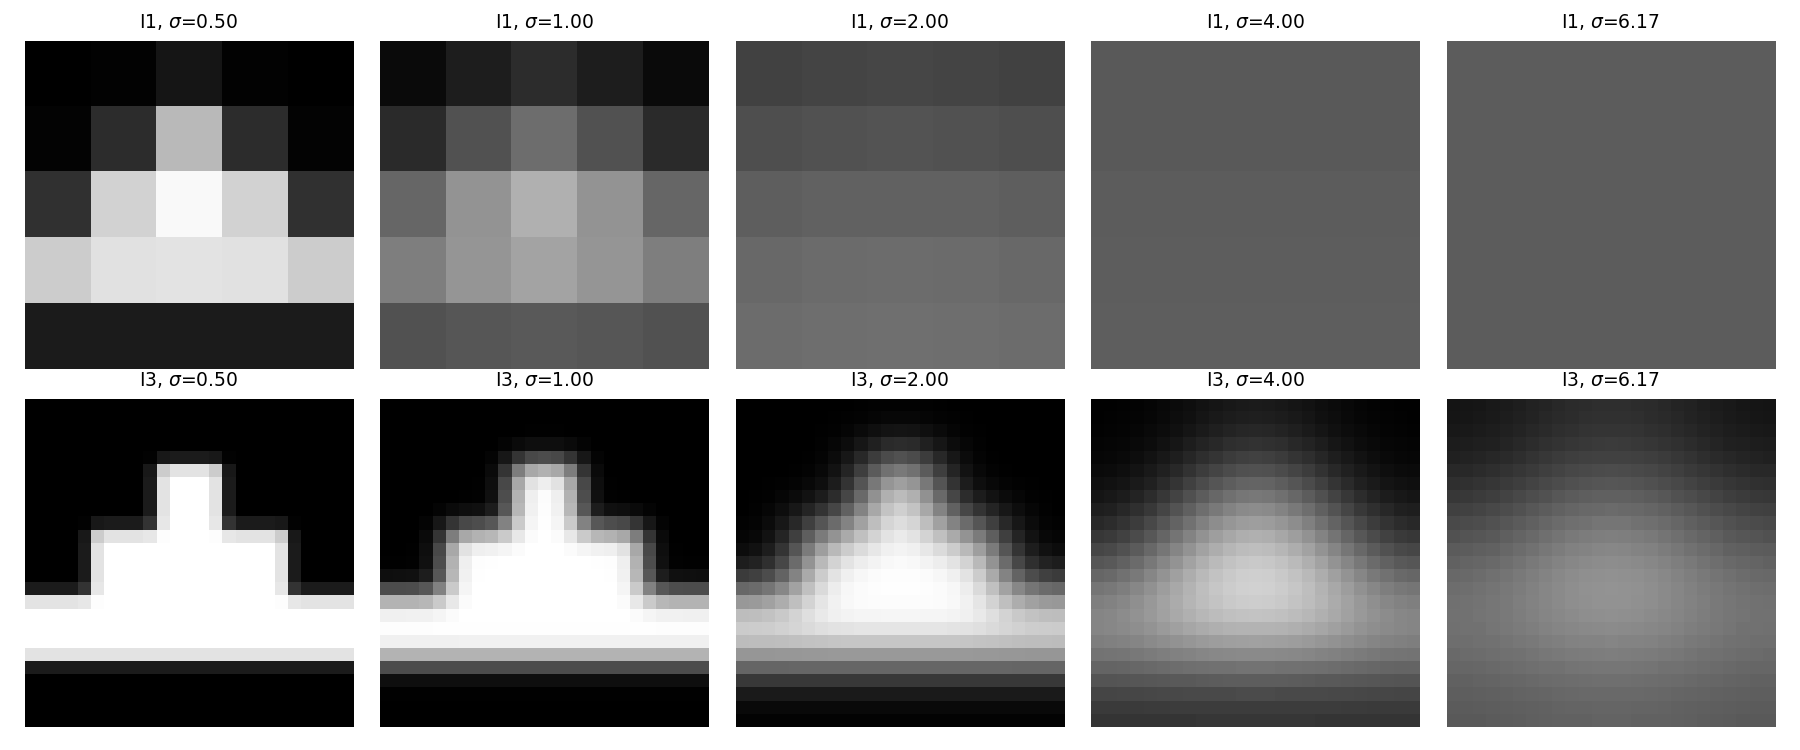
\includegraphics[width=.9\linewidth]{figs/q3_gauss.png}
\caption{Gaussian scale space $L(x,y,\sigma)$ of $I_1$ (top) and $I_3$ (bottom).}\label{fig:g}
\end{figure}
\begin{figure}[H]\centering
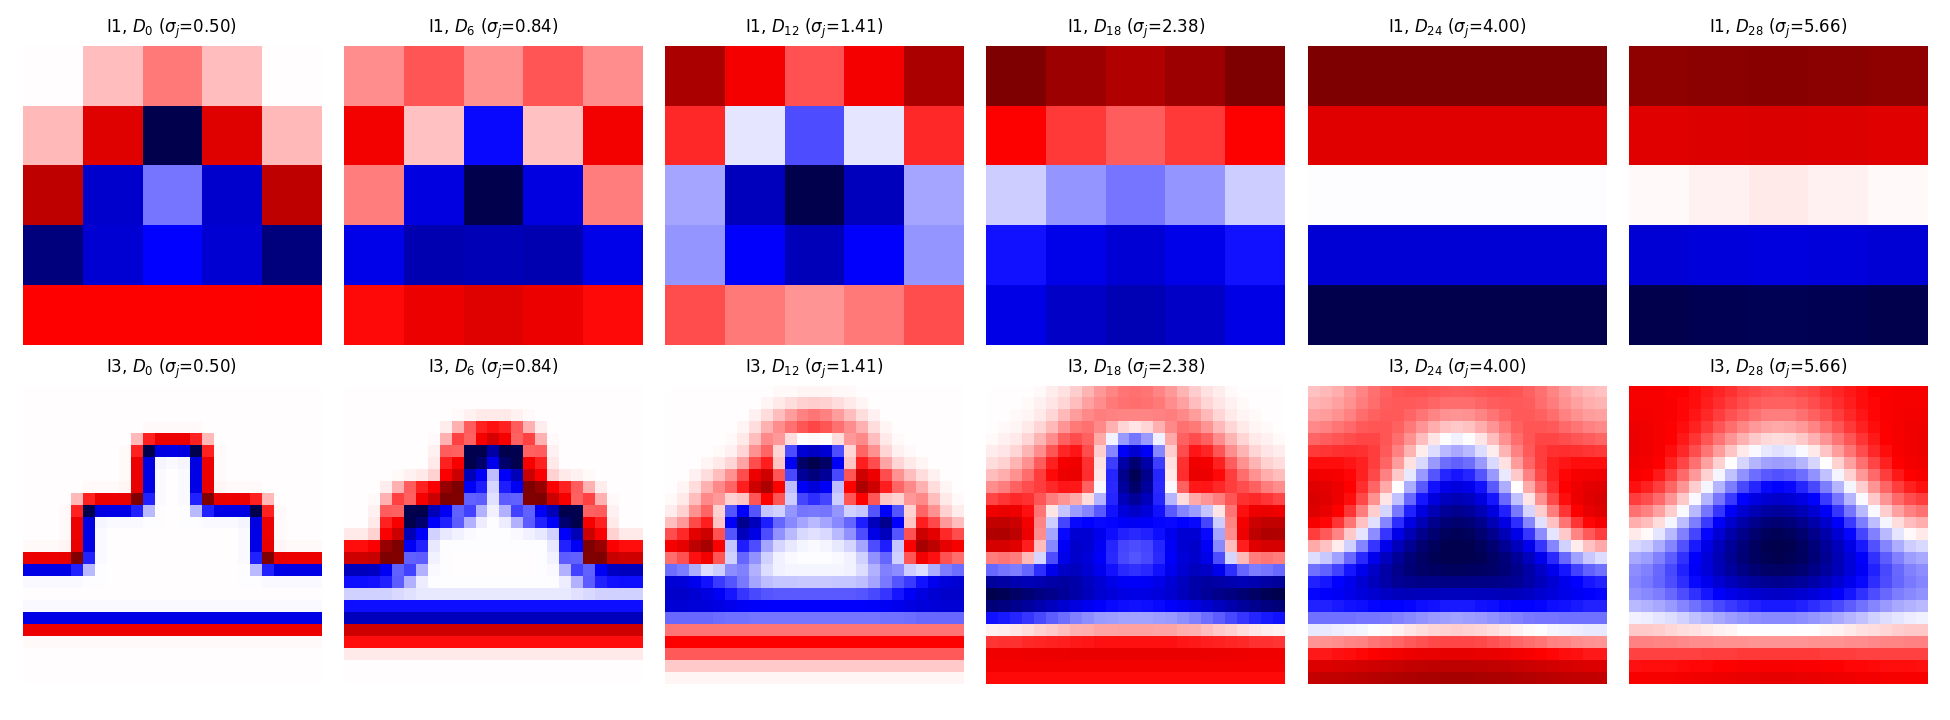
\includegraphics[width=\linewidth]{figs/q3_dog.png}
\caption{DoG images $D_j$ (red $>0$, blue $<0$; each panel uses its own symmetric color scale).}\label{fig:d}
\end{figure}

\textbf{(c)(ii)} Detected extrema (row, col one-based; $D_j$ is labeled by $\sigma_j$):
\begin{center}
\begin{tabular}{llccrl}
\toprule
Image & Location & $j$ & $\sigma_j$ & $D$ & Type\\
\midrule
$I_1$ & (3,3) & 8 & 1.000 & $-10.46$ & min\\
\midrule
$I_3$ & (4,13) & 9 & 1.091 & $+3.66$ & max\\
& (9,9), (9,17) & 10 & 1.189 & $+7.40$ & max\\
& (12,7), (12,19) & 10 & 1.189 & $-7.40$ & min\\
& (14,4), (14,22) & 10 & 1.189 & $+7.45$ & max\\
& (7,13) & 14 & 1.682 & $-8.99$ & min\\
& (14,13) & 26 & 4.757 & $-10.09$ & min\\
\bottomrule
\end{tabular}
\end{center}

\textbf{(iii)} The minimum of $I_1$ at $(3,3)$ and the minimum of $I_3$ at $(14,13)$ both mark the bright triangular blob as a whole. They have the same sign, similar $|D|$, and matching positions: $I_1$ pixel $(r,c)$ maps to $(5r-2,5c-2)$ in $I_3$, so $(3,3)\mapsto(13,13)$, one pixel from the detection.
$\sigma_1=1.000$, $\sigma_3=4.757$.

\textbf{(iv)} $\sigma_3/\sigma_1=4.76\approx5$. The 5\% gap is below one scale step ($2^{1/8}\approx1.09$): the true value 5 lies between the sampled $\sigma=4.757$ and $5.187$. The characteristic scale therefore grows with the enlargement factor, as expected.

\textbf{(v)} The other $I_3$ extrema are small-scale structures, namely the tip ($(7,13)$, $\sigma=1.68$) and the step corners of the staircase ($\sigma\approx1.19$). Their $I_1$ counterparts would sit at $\sigma\approx1.68/5\approx0.34$ and $0.24$, which is below $\sigma_0=0.5$, and some would also be on the 5$\times$5 border. Figure~\ref{fig:tip} confirms this. At the $I_1$ tip, $|D_j|$ is largest at the smallest scale and only decreases, so the peak lies below the sampled range. At the $I_3$ tip, $|D_j|$ peaks at $\sigma\approx1.8$, about 5$\times$ the unresolved $I_1$ scale.
\begin{figure}[H]\centering
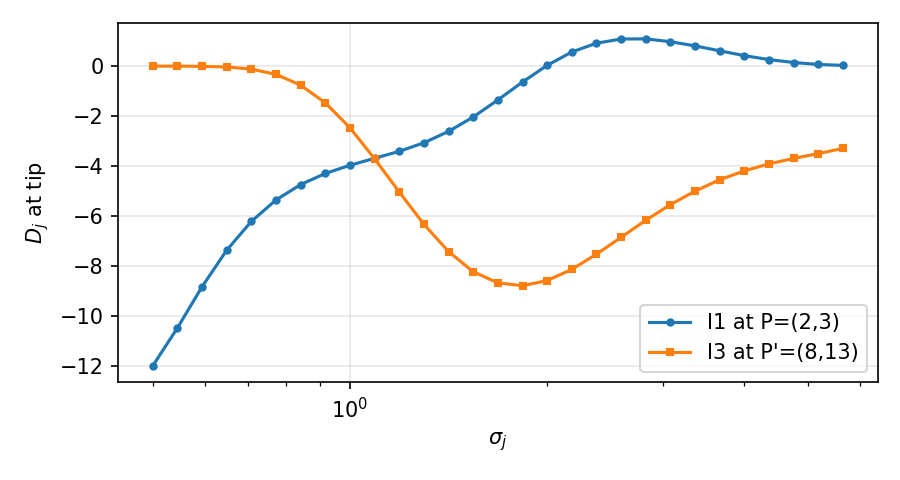
\includegraphics[width=.55\linewidth]{figs/q3_tip_curve.png}
\caption{DoG response at the tip, $I_1$ at $(2,3)$ vs.\ $I_3$ at $(8,13)$.}\label{fig:tip}
\end{figure}

\textbf{(d)} Harris uses one fixed window, so the same structure gives different responses at different image sizes (Problem 2e: $R$ falls from $2.3\times10^7$ to 0). The DoG detector searches over $(x,y,\sigma)$. Since $D\approx(k-1)\sigma^2\nabla^2G*I$ is scale-normalized, the extremum appears at a $\sigma^\ast$ proportional to the structure size. Scale selection thus makes the detection covariant with scale ($\sigma_3/\sigma_1\approx5$).

%=====================================================================
\section*{Problem 4: Homography, DLT and RANSAC}

\textbf{(a)} I selected 20 correspondences (Fig.~\ref{fig:corr}): the 4 black markers (blob centroids) and 16 window/sill corners spread over the facade. Each $I_2$ location was checked by local normalized cross-correlation (NCC $>0.9$). Coordinates are $(u,v)=(\text{col},\text{row})$:
\begin{center}\small
\begin{tabular}{rcc@{\hspace{2em}}rcc}
\toprule
$i$ & $(u_1,v_1)$ & $(u_2,v_2)$ & $i$ & $(u_1,v_1)$ & $(u_2,v_2)$\\
\midrule
1 & (307.1, 233.1) & (245.0, 228.2) & 11 & (154, 134) & (112, 152)\\
2 & (407.0, 230.1) & (351.0, 229.7) & 12 & (435, 117) & (396, 124)\\
3 & (310.1, 280.9) & (245.0, 268.8) & 13 & (312, 79) & (258, 98)\\
4 & (409.7, 274.2) & (350.9, 268.7) & 14 & (380, 146) & (328, 154)\\
5 & (59, 128) & (40, 151) & 15 & (251, 234) & (192, 230)\\
6 & (268, 20) & (217, 51) & 16 & (348, 43) & (299, 62)\\
7 & (180, 264) & (130, 250) & 17 & (84, 87) & (58, 120)\\
8 & (209, 168) & (157, 178) & 18 & (337, 197) & (277, 200)\\
9 & (311, 142) & (254, 153) & 19 & (95, 251) & (66, 239)\\
10 & (246, 107) & (192, 127) & 20 & (266, 279) & (204, 265)\\
\bottomrule
\end{tabular}
\end{center}
\begin{figure}[H]\centering
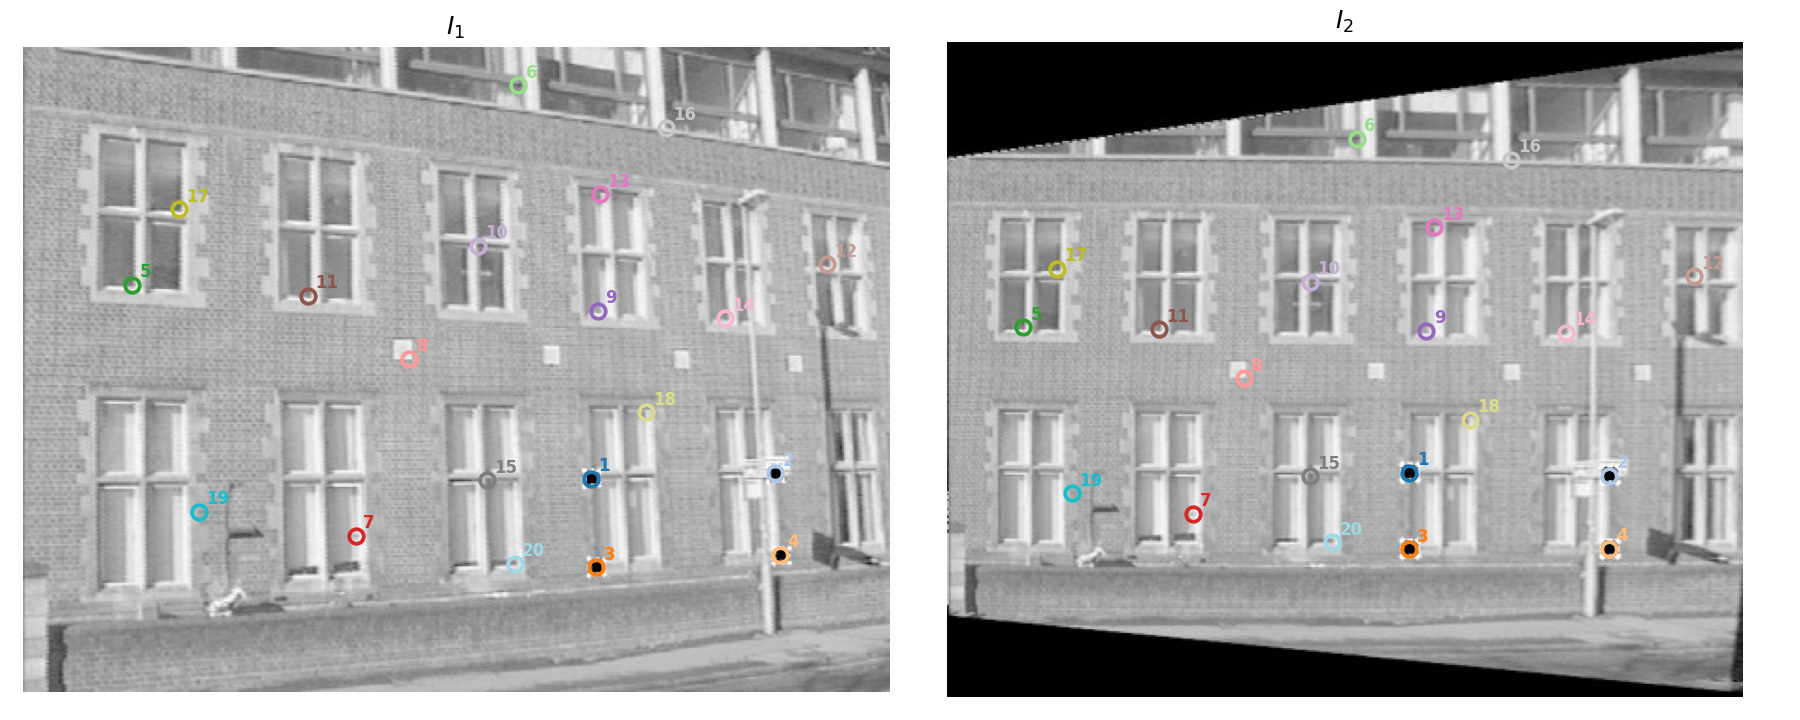
\includegraphics[width=.9\linewidth]{figs/q4a_corr.png}
\caption{20 manual correspondences (same color and number on both images).}\label{fig:corr}
\end{figure}

\textbf{(b)} Each pair contributes two rows of $A\in\mathbb R^{40\times9}$:
\[
[u_1,v_1,1,0,0,0,-u_2u_1,-u_2v_1,-u_2],\qquad [0,0,0,u_1,v_1,1,-v_2u_1,-v_2v_1,-v_2].
\]
The minimizer of $\|Ah\|^2$ subject to $\|h\|=1$ is the right singular vector of $A$ for the smallest singular value. Normalized so that $\sum h_{ij}^2=1$:
\[
H_{\text{DLT}}=\begin{bmatrix}
1.0845\times10^{-2} & 1.1532\times10^{-4} & -1.7605\times10^{-2}\\
-2.1130\times10^{-3} & 1.1942\times10^{-2} & 9.9958\times10^{-1}\\
-1.0475\times10^{-5} & 3.3547\times10^{-6} & 1.6074\times10^{-2}
\end{bmatrix}
\]
The reprojection error is 0.48 px on average and 1.60 px at most.

\textbf{(c)(i)} With a fixed seed, 5 of the 20 correspondences (25\%, $i=2,4,8,9,18$) had their targets replaced by uniformly random pixels in $I_2$ (Fig.~\ref{fig:out}, red).
\begin{figure}[H]\centering
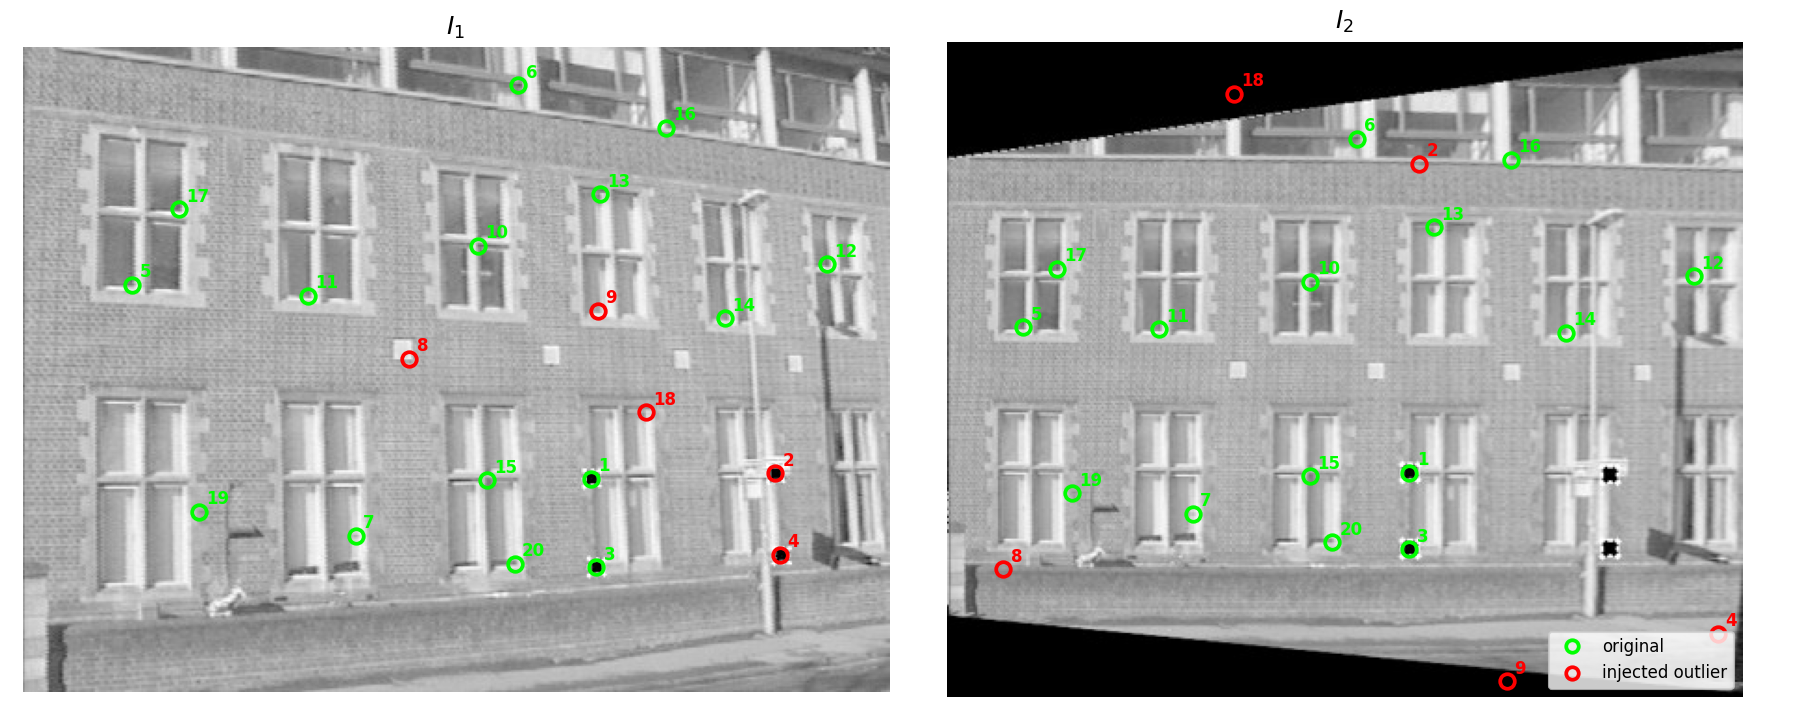
\includegraphics[width=.85\linewidth]{figs/q4c_outliers.png}
\caption{Correspondences after outlier injection (red = injected outliers).}\label{fig:out}
\end{figure}

\textbf{(ii)} DLT on all 20 pairs:
\[
H_{\text{outlier}}=\begin{bmatrix}
-7.9599\times10^{-4} & -2.0679\times10^{-3} & 6.6709\times10^{-1}\\
-1.6073\times10^{-3} & -1.1012\times10^{-3} & 7.4496\times10^{-1}\\
-6.9562\times10^{-6} & -7.5502\times10^{-6} & 3.9259\times10^{-3}
\end{bmatrix}
\]

\textbf{(iii)} Adaptive RANSAC ($s=4$, $\tau=3$ px, $p=0.99$). Start with $N=\infty$. In each iteration: draw 4 pairs (skip degenerate samples with 3 collinear points), fit $H$ by DLT, compute $e_i=\|(u_{2i},v_{2i})-(\hat u_{2i},\hat v_{2i})\|$, and count inliers $e_i<\tau$. When the consensus set improves, set $\epsilon=1-\#\text{inliers}/n$ and update $N=\log(1-p)/\log\!\big(1-(1-\epsilon)^4\big)$. Stop when the iteration count reaches $N$, then re-fit DLT on the largest inlier set.

\textbf{(iv)} The run took \textbf{13 iterations} (final $\epsilon=0.25$ gives $N=12.1$). It found \textbf{15 inliers and 5 outliers}, exactly the injected ones (Fig.~\ref{fig:rs}).
\[
H_{\text{RANSAC}}=\begin{bmatrix}
1.0792\times10^{-2} & 9.5647\times10^{-5} & -1.5552\times10^{-2}\\
-2.1100\times10^{-3} & 1.1846\times10^{-2} & 9.9962\times10^{-1}\\
-1.0433\times10^{-5} & 3.2084\times10^{-6} & 1.6011\times10^{-2}
\end{bmatrix}
\]
\begin{figure}[H]\centering
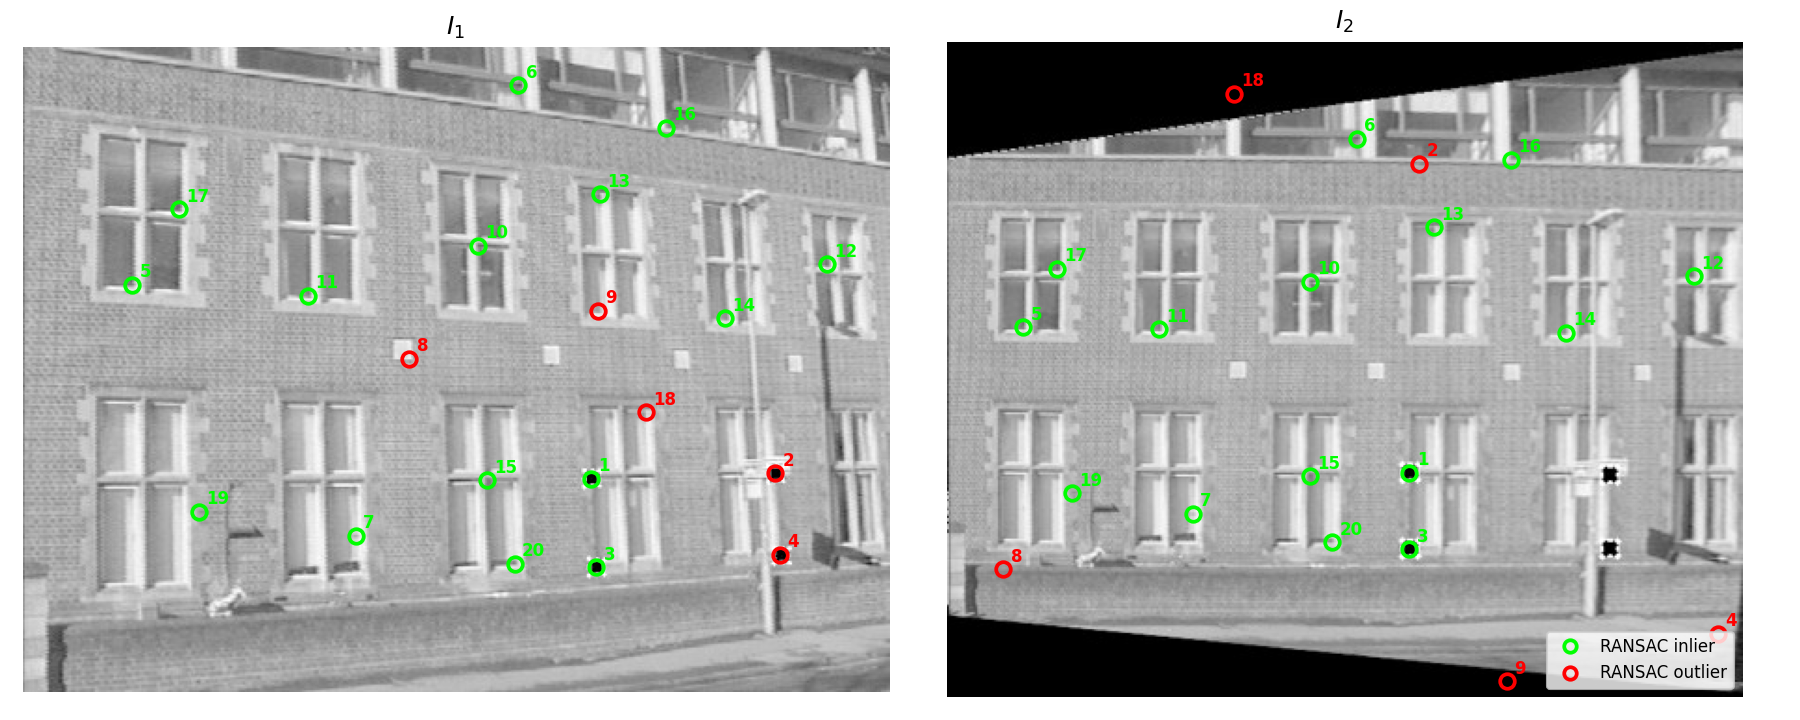
\includegraphics[width=.85\linewidth]{figs/q4c_ransac.png}
\caption{RANSAC classification: green = inliers, red = outliers.}\label{fig:rs}
\end{figure}

\textbf{(d)(i)} Warped images (bilinear interpolation, 0 outside the source) are shown in Fig.~\ref{fig:warp}.
\begin{figure}[H]\centering
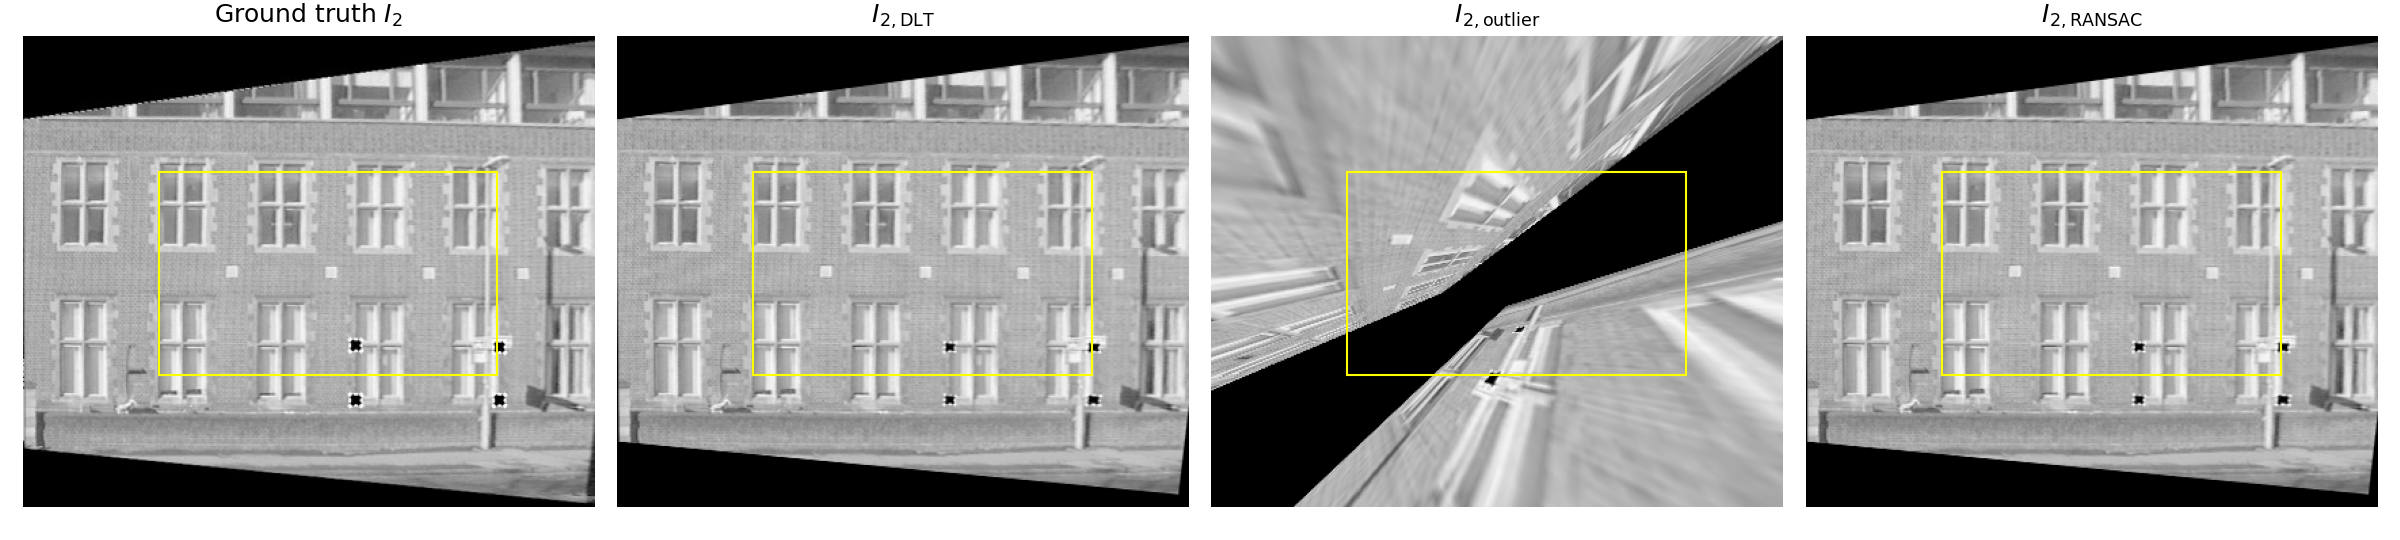
\includegraphics[width=\linewidth]{figs/q4d_warps.png}
\caption{Ground truth $I_2$ and the warps of $I_1$ by $H_{\text{DLT}}$, $H_{\text{outlier}}$ and $H_{\text{RANSAC}}$. The yellow box is $\Omega$.}\label{fig:warp}
\end{figure}

\textbf{(ii)} MSE over $\Omega=\{100\le u\le350,\ 100\le v\le250\}$ (grayscale, 0--255):
\begin{center}
\begin{tabular}{lr}
\toprule
\textbf{Homography Estimation Method} & \textbf{MSE}\\
\midrule
DLT (original correspondences) & 54.14\\
DLT (with outliers) & 13544.20\\
RANSAC + DLT & 57.94\\
\bottomrule
\end{tabular}
\end{center}

\textbf{(iii)} DLT minimizes the summed algebraic error over all pairs, so every correspondence affects the result. A few outliers with errors of hundreds of pixels dominate the least-squares solution and give a completely wrong $H$: MSE rises about 250$\times$, from 54 to 13544, and the warp is unrecognizable. RANSAC fits $H$ from minimal samples and keeps the model with the largest consensus. Outliers are rejected because they disagree with any correct model, and the final DLT uses only the inliers. Its MSE (57.9) is nearly equal to that of clean DLT. The small remaining gap comes from fitting 15 instead of 20 points (less noise averaging); the residual MSE comes from interpolation, JPEG artifacts and sub-pixel errors in the selected points.

\end{document}
